\documentclass[11pt]{article}
\usepackage[letterpaper,margin=.85in]{geometry}
\usepackage[T1]{fontenc}\usepackage{lmodern}\usepackage{microtype}
\usepackage{booktabs,longtable,enumitem,amsmath,graphicx}
\usepackage[bookmarksnumbered,bookmarksopen,pdftitle={Circling Dragons: Map Design and Current Rules Concept}]{hyperref}\usepackage{url}
\usepackage{tikz}
\usepackage{xcolor}
\definecolor{darkred}{rgb}{0.55,0,0}
% link and heading colors, from CPVI/shared-tex/prolog-article.tex
\definecolor{myTeal}{RGB}{0, 128, 128}
\definecolor{myBlue1}{RGB}{75, 99, 175}
\hypersetup{
    colorlinks=true,
    linkcolor=myBlue1,
    filecolor=magenta,
    urlcolor=cyan,
    citecolor=myTeal
}
\usepackage{sectsty}
\sectionfont{\color{myBlue1}}
\subsectionfont{\color{myBlue1}}
\subsubsectionfont{\color{myBlue1}}

% Copyright Ben Paul Wise. All Rights Reserved.
% The full-page locator map before each section of figures: the standard sheet with the area of the section's
% figures boxed in black.  Shared by circling_dragons_map_and_rules_V3.tex and maneuver_studies_75km.tex; needs
% graphicx and tikz.  The boxes are generated by map_graphics/xml/tools/cd/illustrate.py (locator-boxes.tex).
% The map is set once in a box, so the PDF carries one copy of the image however many locators there are.
% Copyright Ben Paul Wise. All Rights Reserved.
% Generated by map_graphics/xml/tools/cd/illustrate.py; do not edit.  The area each section's figures show
% on the standard sheet, as a TikZ rectangle in fractions of the sheet (x from the left, y from the bottom).
\def\cdboxIchigo{(0.1568,0.0943) rectangle (0.5986,0.6013)}   % 1-ichigo-setup
\def\cdboxReflux{(0.1568,0.0943) rectangle (0.5986,0.6013)}   % 2-reflux-setup
\def\cdboxAugust{(0.3402,0.5942) rectangle (0.9654,0.9891)}   % 3-august-setup
\def\cdboxRace{(0.2587,0.4484) rectangle (0.8432,0.9241)}   % 4-race-setup
\def\cdboxChangsha{(0.3198,0.2297) rectangle (0.4968,0.3746)}   % a1-changsha-position
\def\cdboxHengyang{(0.2995,0.1568) rectangle (0.4764,0.3225)}   % b1-hengyang-position
% Copyright Ben Paul Wise. All Rights Reserved.

\newsavebox{\cdmapbox}
\AtBeginDocument{\sbox{\cdmapbox}{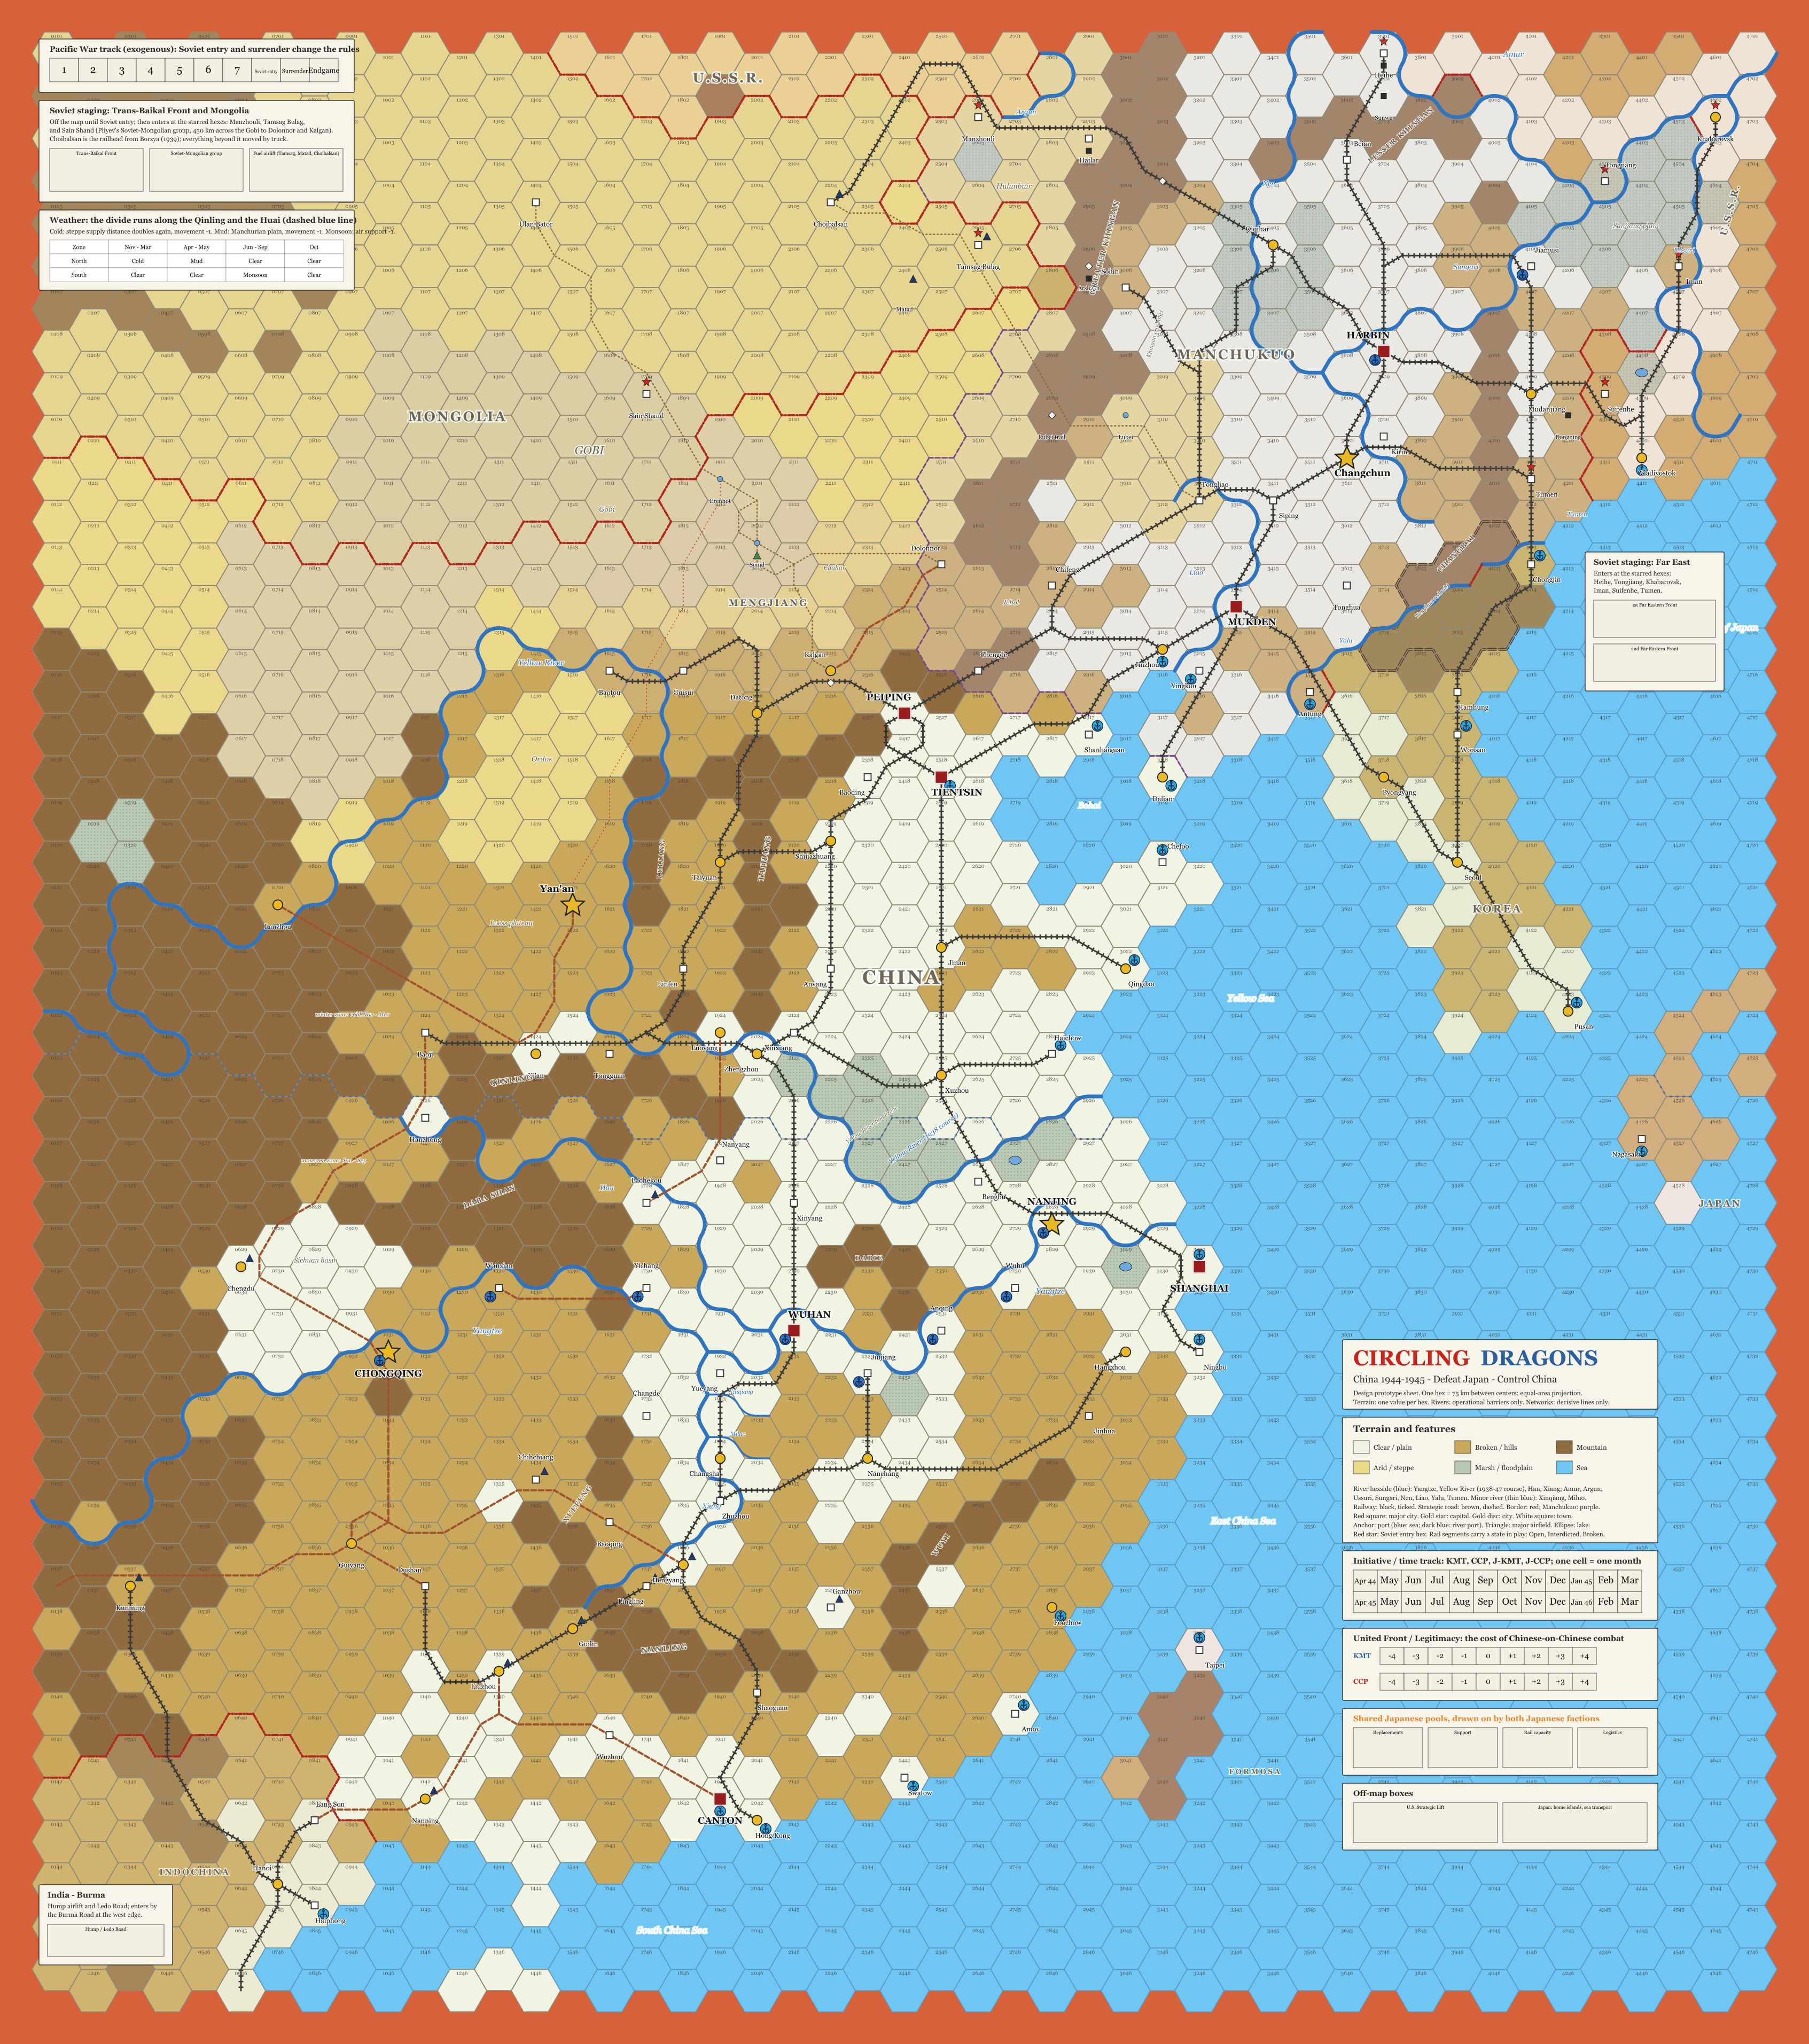
\includegraphics[width=\textwidth,height=.84\textheight,keepaspectratio]{../map_graphics/xml/circling-dragons.png}}}
\newcommand{\locator}[2]{%
  \clearpage
  \begin{figure}[p]\centering
  \begin{tikzpicture}
    \node[anchor=south west,inner sep=0] (map) at (0,0) {\usebox{\cdmapbox}};
    \begin{scope}[x={(map.south east)},y={(map.north west)}]
      \draw[white,line width=5pt] #1;
      \draw[black,line width=2.6pt] #1;
    \end{scope}
  \end{tikzpicture}
  \caption{#2}
  \end{figure}
  \clearpage}
% Copyright Ben Paul Wise. All Rights Reserved.

\setlist{nosep}
\title{\textbf{Circling Dragons}\\\large Map Design and Current Rules Concept\\\normalsize China, 1944--1945}
\author{}\date{Draft design memorandum, version 3 --- October 2026}
\begin{document}
\begin{titlepage}
\centering
\vspace*{\fill}
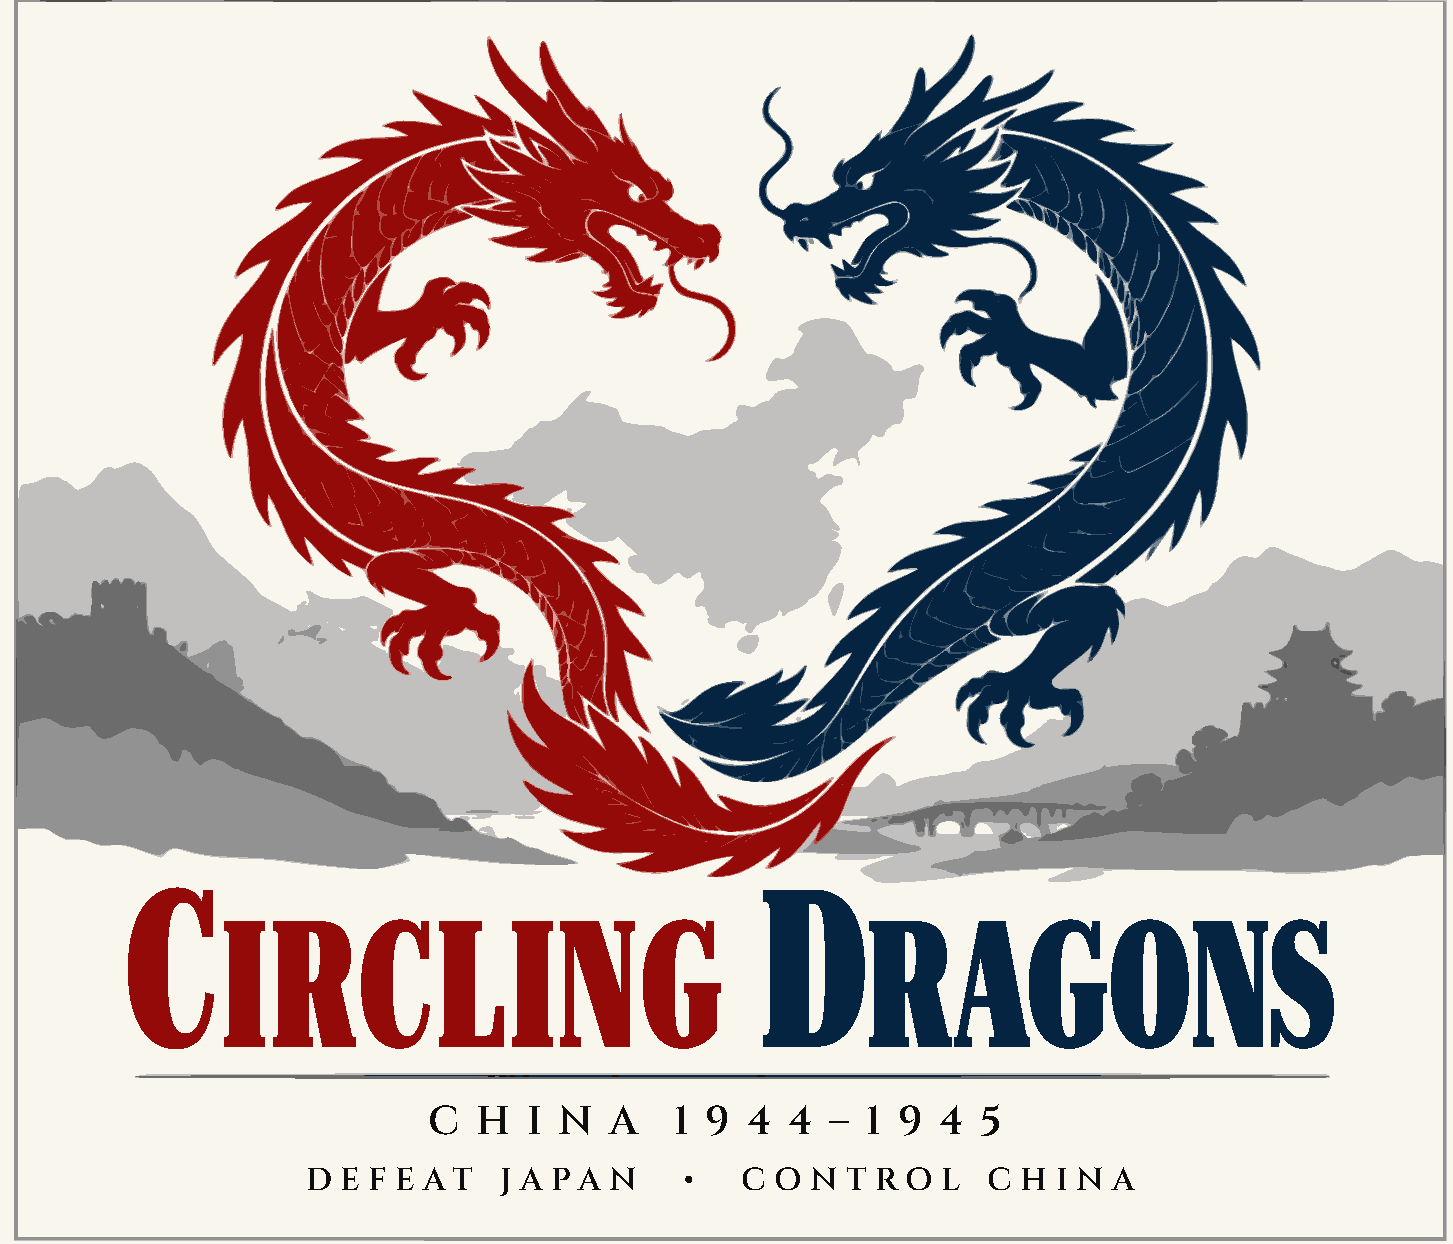
\includegraphics[width=.92\textwidth]{circling-dragons-logo-V2.pdf}
\vspace*{\fill}
\end{titlepage}
\maketitle
\begin{abstract}
This memorandum develops a map and rules architecture for \emph{Circling Dragons}, a two-player strategic-operational game about defeating Japan in China while the KMT and CCP position themselves for the renewed Chinese Civil War. It adapts the crossed-control idea of \emph{Battle for Germany} and \emph{Downfall}: each player commands his own Chinese faction and the Japanese forces principally opposing the other Chinese faction. Historical geography suggests that the board should be a sparse transportation network laid over coarse terrain barriers, rather than a conventional terrain map covered with minor roads and tactical detail.

{\bfseries\footnotesize\color{darkred}This is an AI-generated experimental text, not to be
distributed without written permission.}
\end{abstract}
\clearpage
\begingroup\small\tableofcontents\endgroup
\clearpage

\section{Design conclusions}
\begin{enumerate}
\item The game builds on the ``two players, four factions'' system of \emph{Downfall} to represent Mao Zedong and Chiang Kai-shek cooperating to defeat the Japanese while each positions his faction for the coming civil war.
\item The map uses \textbf{75 km per hex}. The first sheet used 100 km, close to \emph{Downfall}'s 110 km land hexes; at that scale the Hunan corridor was too narrow for the defender's maneuver (section~\ref{sec:maneuvers}).
\item The game keeps an operational focus and does not force players into excessive tactical detail. Railways, major river crossings, strategic roads, ports, airfields, and mountain corridors matter more than fine terrain differentiation.
\item The game uses a continuous initiative/time track similar to that of \emph{Downfall}; a full calendar interval is about one month.
\item KMT and Japanese power is primarily conventional control of nodes and communications. Much CCP power is rural \emph{presence/base control}, capable of interdiction and political expansion.
\item Manchuria has enough space for the Soviet western, eastern, and northeastern approaches.
\item The August 1945 surrender changes the phase of the game: Japanese combat power declines, and railways, ports, cities, surrender sites, and access to Manchuria become the principal objectives.
\end{enumerate}

\section{Terrain and operational geography}
The map uses five terrain types, \textbf{clear/plain, broken/hills, mountain, marsh/floodplain, and arid/steppe}, with the waterless desert of the Gobi and the Alashan as a variant of steppe. Forest is normally included in broken or mountain terrain. The objective is operational canalization, not tactical simulation.

\subsection{Rivers}
The map prints the \textbf{Yellow River} and the \textbf{Yangtze} as major barriers, and the Han and the Xiang where they shape campaign corridors. In Manchuria, the \textbf{Amur, Ussuri, Sungari/Songhua, Nen, Liao, and Argun} systems matter because they define floodplains, crossings, and operational axes. Minor tributaries are represented by terrain costs, with one exception: the standard sheet prints two \textbf{minor rivers}, the Xinqiang and the Miluo north of Changsha, because they were the delay lines of the Changsha battles (section~\ref{sub:sheet75}).

\subsection{Mountains}
The map makes the \textbf{Taihang}, \textbf{Qinling/central belt}, \textbf{Xuefeng}, \textbf{Nanling/Guangxi-Guizhou broken terrain}, \textbf{Greater Khingan}, \textbf{Lesser Khingan}, and eastern Manchurian highlands visually obvious. The Xuefeng barrier shaped the 1945 Chihchiang/West Hunan campaign. The Greater Khingan is especially important (Glantz, \emph{August Storm}): Japanese planning treated it and its few routes as a major barrier, and the Soviet operational surprise depended partly on crossing terrain that the defense underestimated.

Only a few passes are named. Usually a railway or strategic road crossing a mountain hex represents a pass.

\subsection{Marsh and steppe}
Marsh is rare in China proper but prominent in northeastern Manchuria, especially on the Amur--Ussuri--Sungari floodplain. The steppe and desert of western Manchuria and Mongolia penalize supply more than combat.

\section{Transportation as the structure of the board}
The map follows one cartographic rule:
\begin{quote}\textbf{A transportation line is printed only if removing it would change a player's strategic decisions.}\end{quote}

The core rail network includes:
\begin{itemize}
\item \textbf{Peiping--Hankow (Pinghan)}, central to the first phase of Ichi-Go;
\item \textbf{Canton--Hankow/Hunan corridor}, especially Changsha--Hengyang;
\item \textbf{Hunan--Guangxi}, Hengyang--Guilin--Liuzhou;
\item \textbf{Longhai}, the main east--west trunk of the central plains;
\item \textbf{Tientsin--Pukow (Jinpu/Tsinpu)};
\item \textbf{Peiping--Suiyuan, Datong--Puzhou, and Shijiazhuang--Taiyuan};
\item \textbf{Manchurian trunks}: Harbin--Changchun--Mukden, the South Manchuria line, Harbin--Qiqihar--Hailar/Manzhouli, and the eastern line through Mudanjiang to Suifenhe; and
\item \textbf{Shanhaiguan corridor}, the overland gateway between North China and Manchuria.
\end{itemize}

The post-surrender political record supports this emphasis: the negotiations of 1945 concerned the major railway zones explicitly (FRUS 1945, vol.~VII; section~\ref{sec:sources}), so rail control enters the victory and political systems as well as movement.

The map does not print a dense road net. It prints only the \textbf{Strategic Roads} whose existence changes supply or connects otherwise difficult terrain. The Yangtze and the Sungari provide limited strategic transport between designated ports.

\section{Operational nodes}
A city appears on the map if it is a transport junction, a political objective, a major port or airfield, or the base of a campaign.

\begin{longtable}{p{.23\textwidth}p{.69\textwidth}}
\toprule Node & Map function \\\midrule\endhead
Peiping--Tientsin & Political/transport center; ports and railheads; a principal objective of the 1945 surrender race.\\
Shijiazhuang--Taiyuan & Taihang rail corridor; Japanese occupation and CCP interdiction geography.\\
Zhengzhou & Junction of major north--south and east--west rail axes; objective of the first phase of Ichi-Go.\\
Wuhan & Yangtze transport hub and northern base of the central Ichi-Go corridor.\\
Changsha--Hengyang & Main Hunan corridor; major 1944 fighting and transport/airfield objectives.\\
Guilin--Liuzhou & Southern Ichi-Go rail and airfield objectives.\\
Chihchiang (Zhijiang) & 1945 airfield objective west of the Xuefeng barrier.\\
Chongqing/Chengdu & KMT political/rear-area center, near the western edge of the map.\\
Yan'an & CCP political/base node rather than conventional logistics hub.\\
Shanghai--Nanjing & Political, industrial, port and rail objectives.\\
Qingdao/North China ports & Strategic entry points for post-surrender transport.\\
Shanhaiguan--Qinhuangdao & Narrow gateway and rail connection into Manchuria.\\
Mukden, Changchun, Harbin & Principal central/southern Manchurian political and rail hubs.\\
Qiqihar, Hailar/Manzhouli & Northwestern communications and approach nodes.\\
Mudanjiang/Suifenhe & Eastern road/rail axis and major Soviet-Japanese corridor.\\
Dalian/Port Arthur; Huludao/Yingkou & Ports affecting entry into southern Manchuria.\\
\bottomrule
\end{longtable}

\section{Map extent and density}
The map uses \textbf{75 km per hex} and allows modest distortion where it preserves the topology of junctions and corridors. It extends from Mongolia/Soviet territory and Manchuria in the north to Guangxi/northern Indochina in the south, and from the coast west to the Chongqing--Chengdu/Shaanxi rear areas.

Remote western China is compressed or handled with off-map boxes, so that the board area goes to the contested corridors. Two map sheets, as in \emph{Downfall}, suffice: at 3/4 inch hexes the sheet is about 32 by 36 inches.

\subsection{The standard sheet at 75 km}\label{sub:sheet75}
% Copyright Ben Paul Wise. All Rights Reserved.
% The standard sheet at 75 km: shared by circling_dragons_map_and_rules_V3.tex and maneuver_studies_75km.tex,
% each of which gives the heading.  Needs the labels sec:maneuvers and sub:mrules (maneuver-studies.tex).
The standard sheet has 75 km between hex centers. It replaced the first sheet, at 100 km, in October 2026, because at 100 km the Hunan corridor is too narrow for two maneuvers that decided its battles: Xue Yue's defense of Changsha in 1939--42 and the Japanese envelopment of Hengyang in 1944 (section~\ref{sec:maneuvers}).

Both sheets cover the same area and are built by the same programs from the same sources, so the scale is a setting of the build and the first sheet can still be produced for comparison. Every ruling made on the 100 km sheet was carried over: the named mountain ranges, the lakes and the Tonghua redoubt are lists of 100 km hexes, and each 75 km hex whose center falls in a listed hex takes the ruling. Three coastal hexes, each just under half land, were ruled land so that the railways of the Liaodong peninsula, the south shore of Hangzhou Bay and the Korean west coast stay on land. At Yueyang the Yangtze was moved to the north side of the city's hex, so that the railway south to Changsha does not cross it. Between Tongguan and Zhengzhou the Yellow River was moved to the north side of the Sanmenxia and Luoyang hexes, so that the Longhai railway stays on the south bank and crosses the river only on its 1938--47 course east of Zhengzhou. The Ussuri was extended two hexsides to join the Amur at Khabarovsk. The sheet passes the same validation and network checks as the first one.

\begin{center}
\begin{tabular}{lrr}
\toprule & First sheet & Standard sheet \\\midrule
Distance between hex centers & 100 km & 75 km \\
Columns by rows & 35 by 34 & 47 by 46 \\
Hexes on the sheet & 1,190 & 2,162 \\
Hexes in play (China, Manchukuo, Korea) & 672 & 1,187 \\
Mongolian hexes, open to Soviet formations only & 131 & 242 \\
Clear hexes across the corridor at Changsha & 2 & 3 \\
Clear hexes across the corridor at Hengyang & 2 & 3 \\
Hexes from Yueyang to Changsha & 1 & 2 \\
Hexes from Hankow to Dushan along the corridor & 12 & 15 \\
Sheet size with 3/4 inch hexes & 24 by 27 in & 32 by 36 in \\
\bottomrule
\end{tabular}
\end{center}

Of the hexes in play, the two sheets have nearly the same terrain: clear 26 and 27 percent, broken 33 and 32, mountain 24 and 23, steppe 15 and 15, marsh 3 and 3. The smaller hex does not make the country look flatter, so the terrain thresholds were left unchanged.

The standard sheet adds one line class, the \textbf{minor river}, drawn thinner than the major rivers and printed only where a minor river shaped a campaign. Two are printed: the Xinqiang and the Miluo, the delay lines north of Changsha on which Xue Yue's screens stood. Each crosses the railway column and the lane east of it, and each runs into the Xiang. The Laodao, the third of his lines, lies inside the Changsha hex and is not printed. In the provisional rules a minor river costs less to cross than a major river, and a formation behind one may withdraw before combat (section~\ref{sub:mrules}).

At 3/4 inch hexes the sheet is about 32 by 36 inches and fits on two 22 by 34 inch map sheets joined along their long edges. To keep the density of pieces of the first estimate, the counter set was grown to 126 unit pieces and 250 counters in all.

\begin{figure}[p]\centering
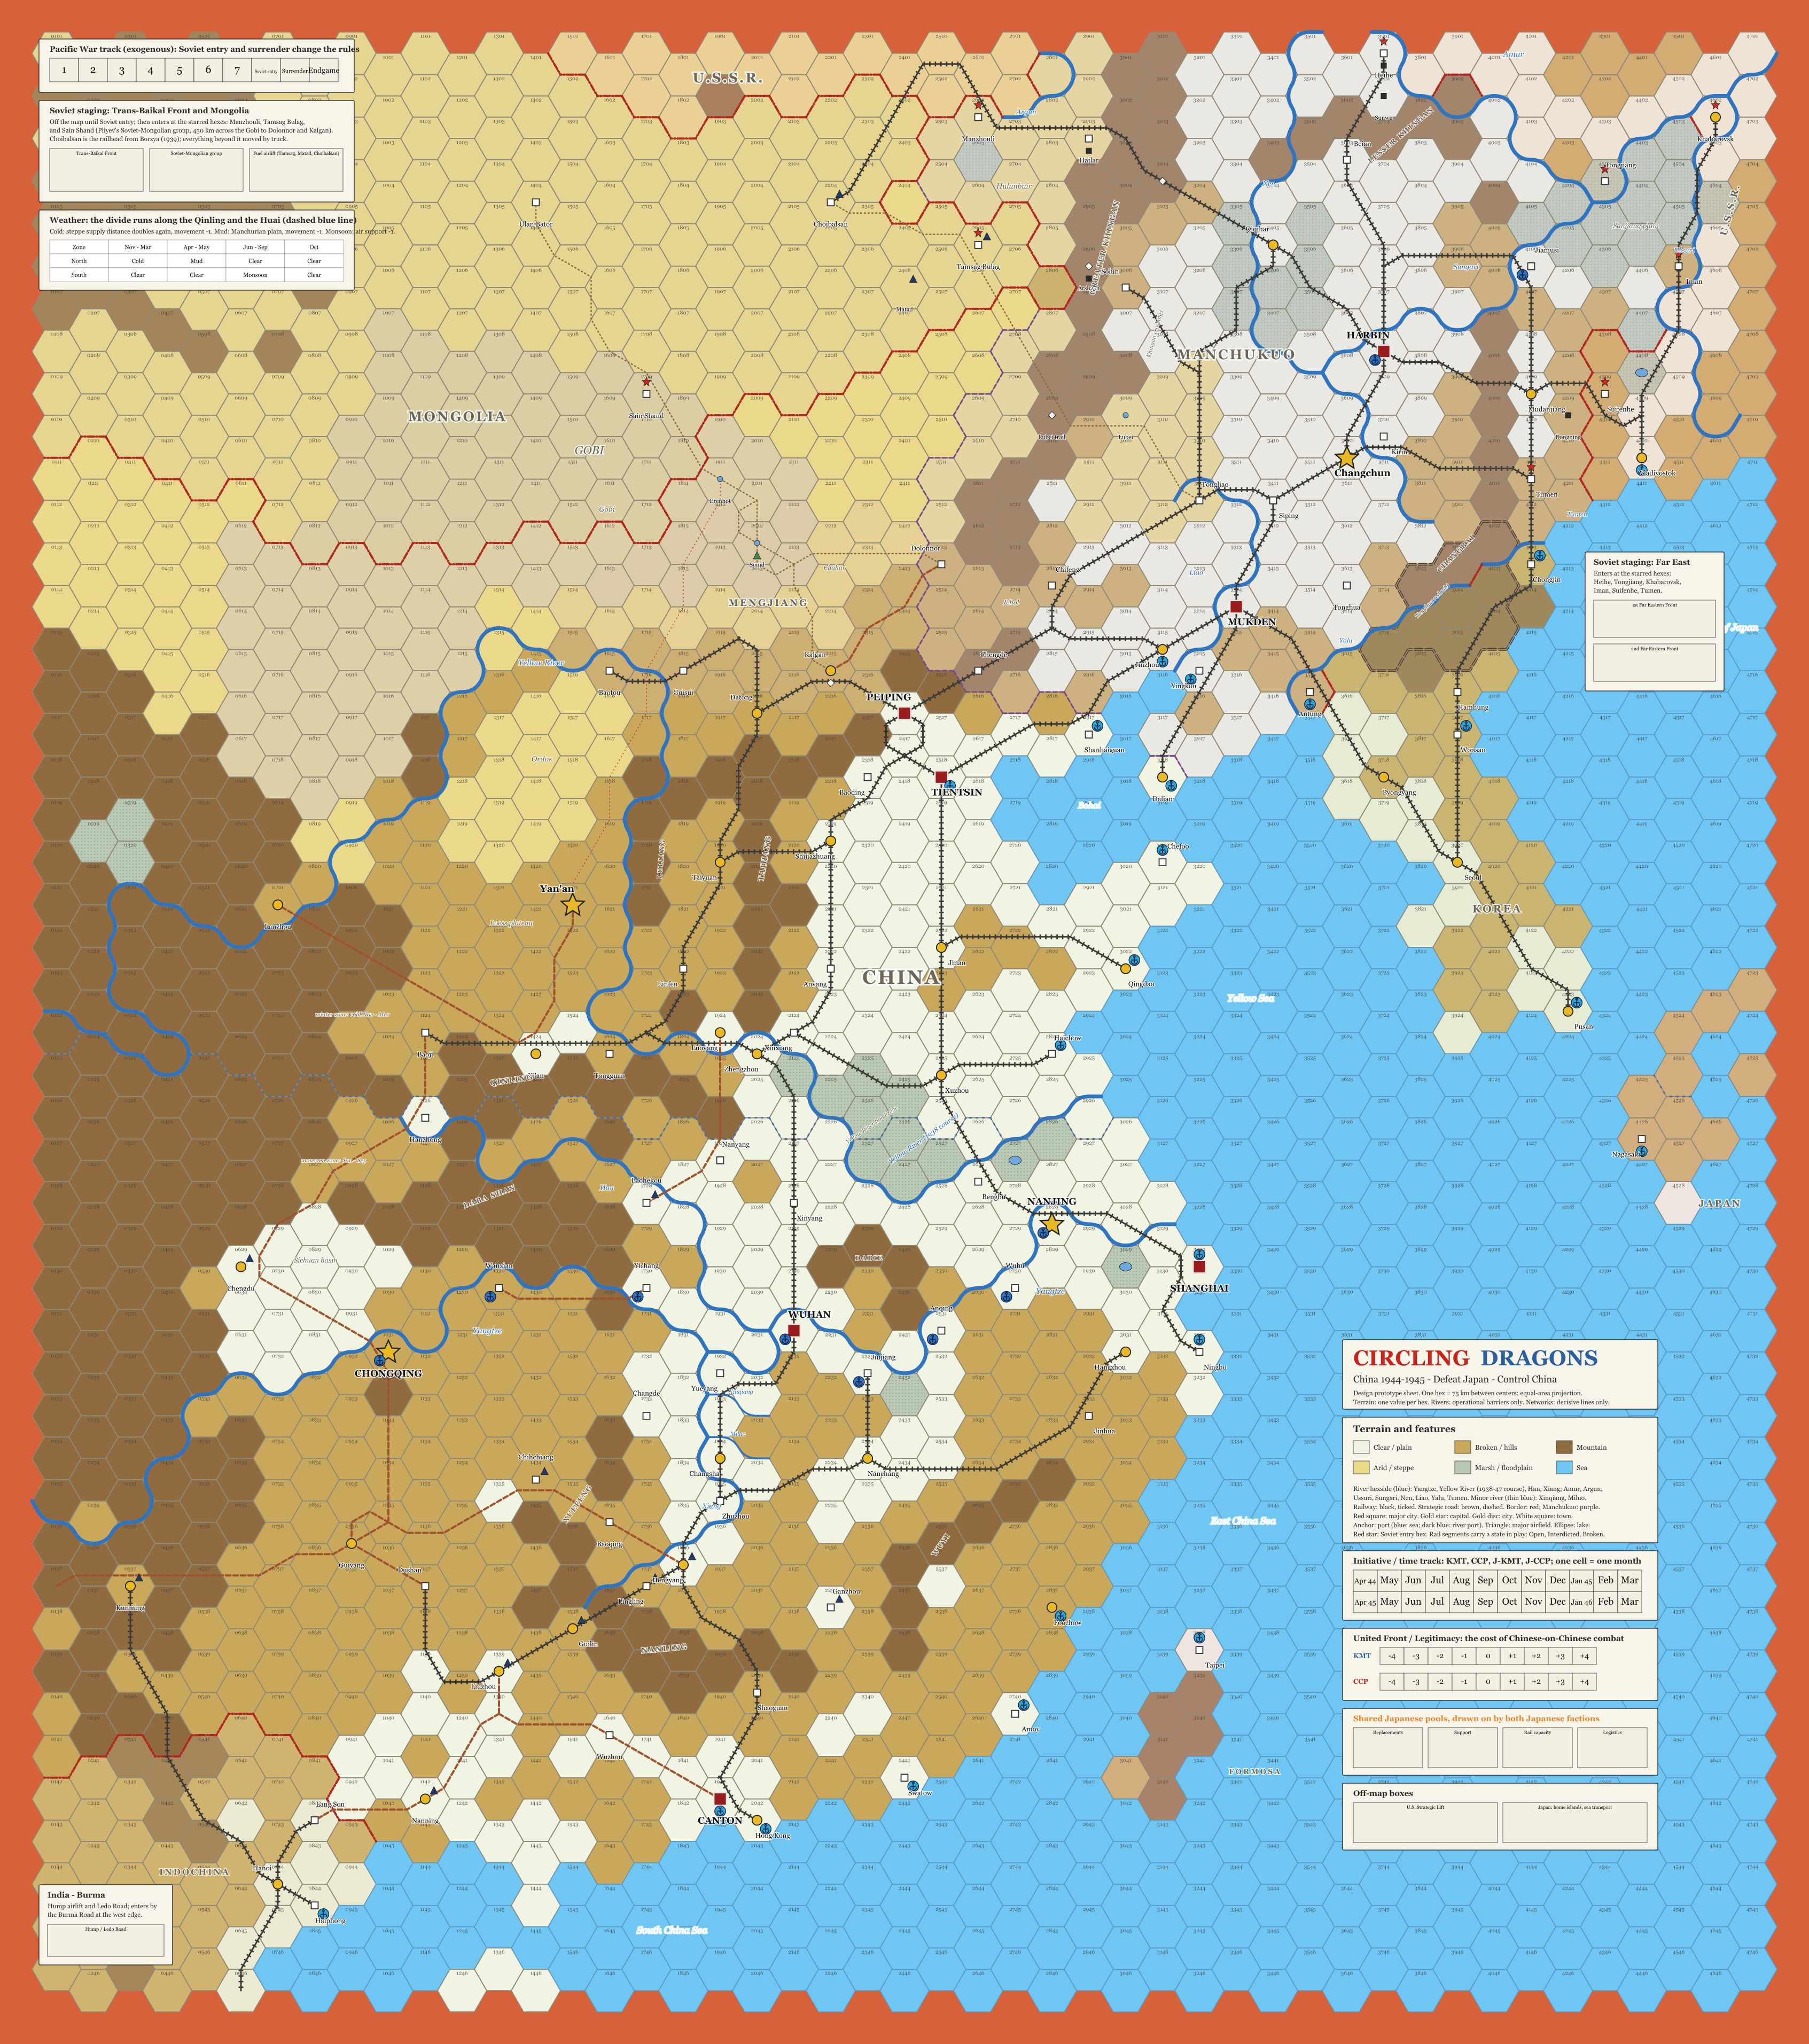
\includegraphics[width=\textwidth,height=.86\textheight,keepaspectratio]{../map_graphics/xml/circling-dragons.png}
\caption{The standard sheet, 75 km between hex centers. The furniture panels keep their size and their places in the corners where little fighting took place; the Mongolian features and the political layer are those of the first sheet.}
\end{figure}
% Copyright Ben Paul Wise. All Rights Reserved.


\section{How the map changes the game}
The original four-faction concept treated KMT, CCP, Japan-against-KMT, and Japan-against-CCP nearly symmetrically. The geography does not support that symmetry, for the reasons below.

\subsection{Conventional and dispersed control}
KMT and Japanese conventional formations depend heavily on rail/strategic-road supply, major junctions, river crossings and operational corridors. CCP power has two layers:
\begin{enumerate}
\item conventional field formations; and
\item \textbf{Base/Presence markers} representing rural political-military control.
\end{enumerate}
Presence can interdict railways, make occupation costly, generate recruitment/political control, and survive loss of a nearby city more readily than a conventional army. Sufficient presence may concentrate into a field formation. The second layer keeps the guerrilla and political dimension of the war in the game at the 75 km hex scale.

\subsection{Rail state}
Rail segments have three states:
\begin{enumerate}
\item \textbf{Open}: supply and strategic redeployment allowed.
\item \textbf{Interdicted}: supply possible with penalty; strategic redeployment blocked or costly.
\item \textbf{Broken}: unusable until repaired.
\end{enumerate}
CCP presence makes interdiction comparatively easy; secure conventional occupation is needed to keep major junctions reliably open.

\section{Current best rules}

\subsection{Players and crossed control}
\begin{center}
\begin{tabular}{lll}
\toprule Player & Own faction & Japanese faction controlled \\\midrule
KMT player & KMT/NRA & Japanese forces principally opposing CCP \\
CCP player & CCP forces & Japanese forces principally opposing KMT \\
\bottomrule
\end{tabular}
\end{center}
Neither player ``is Japan.'' Japanese formations can change controlling player when formally reassigned to a different principal front. Anti-sabotage restrictions prevent a departing controller from deliberately leaving a formation unable to survive.

\subsection{Initiative and time}
There are four initiative markers:
\[
KMT,\qquad CCP,\qquad J_{KMT},\qquad J_{CCP}.
\]
The faction furthest behind on the time track normally acts next. Orders consume different amounts of time. Calendar thresholds trigger seasonal effects and dated strategic events. One calendar interval is approximately one month.

\subsection{Orders}
The menu of orders is short: \textbf{Move/Redeploy, Attack, Move--Attack, Rail Redeploy, Recover/Refit, Political/Base Action,} and \textbf{Interdict/Repair Transport}. Japanese Strategic Directives restrict the objectives their operations may pursue without dictating the exact move.

\subsection{Supply and combat}
A conventional formation traces a short local path to an open railway, strategic road, or eligible river route, then through that network to a supply source. Mountain, marsh and arid terrain sharply restrict off-network supply. Supply matters more than small terrain combat modifiers.

CCP dispersed presence uses a lighter support rule and does not require an unbroken conventional rail chain.

Combat remains highly abstract. Formations have few strength steps. Terrain, supply, support and concentration modify combat. Results are primarily loss, retreat/displacement, disruption, loss of a node, and advance. Mountain and river barriers work mainly by limiting concentration and sustainment rather than by accumulating tactical modifiers.

\subsection{Piece scale and counts (preliminary)}\label{sub:pieces}
The counts below are an estimate, taken from \emph{Downfall}'s density of pieces per hex in play, and the prototype will revise them. \emph{Downfall} prints about 800 land hexes in play and opens with about 90 land pieces on the map, one per nine hexes, rising to about 110 at its peak; its 3--4 step unit is an army, its 2-step unit a corps, its 1-step unit a division. The standard \emph{Circling Dragons} sheet has 1,187 land hexes in play (China proper 895, Manchukuo 247, Korea 45) and 242 Mongolian hexes open to Soviet formations only. The first estimate, made for the 100 km sheet's 672 hexes in play, was 72 unit pieces and about 200 counters; for the 75 km sheet the set was grown to 126 unit pieces and 250 counters.

\begin{center}
\begin{tabular}{lrp{.58\textwidth}}
\toprule Faction & Pieces & What a piece is \\\midrule
Japan & 51 & China Expeditionary Army: 24 division pieces of 3 steps (23 infantry and the 3rd Tank Division), 4 pieces of independent mixed brigades, 7 one-step railway garrisons, and 3 headquarters, the area army a formation answers to deciding the front it faces; Kwantung Army 10 pieces of 2 steps, two for each of its five armies; Korea 3. Reinforced by event in 1945.\\
KMT & 35 & 24 group-army pieces of 2--3 steps and uneven quality, 6 of them regional troops; 5 US-equipped armies, 2 of them in Burma at the start; 2 Y-Force group armies returning from Burma in 1945; 4 headquarters.\\
CCP & 23 & 16 field forces of 2 steps (Eighth Route Army 8, New Fourth Army 7, South China 1); 5 Northeast columns formed in play by concentration of presence; 2 headquarters. Also 24 presence markers whose backs are base areas, which are not pieces.\\
Soviet & 11 & scripted groupings entering in August 1945.\\
Puppets & 6 & Nanjing regime 3, Manchukuo 2, Mengjiang 1; one step each, passing at the surrender.\\
\bottomrule
\end{tabular}
\end{center}

About 105 of the 126 pieces are on the map at the start, one to 11 hexes in play; with the Soviets and the Northeast columns the peak is 126, one to 9.4 hexes, \emph{Downfall}'s density. The piece is therefore \emph{Downfall}'s 2- and 3-step corps-level unit, not its army: at army scale Japan would field 12 pieces and the KMT's twelve war areas 12, too thin for a 47 by 46 sheet. With 5 air-support pieces and 119 markers the counter set comes to 250, against \emph{Downfall}'s 351. A marker with two states carries one on each face: presence and base area, KMT and CCP control, rail interdicted and broken, port denied and open, airfield captured and destroyed, and the front a Japanese formation faces. \textbf{Preliminary:} every figure here is to be tested against the questions in the last section, in particular whether the CCP presence layer stays legible.

\subsection{Shared Japanese resources and directives}
The two Japanese factions draw on shared pools of operational support, replacements, rail capacity, and logistical support. Spending Japanese resources to damage one's Chinese rival therefore reduces what remains for Japanese forces controlled by that rival. Japan therefore remains a single belligerent with one set of resources despite the crossed local control.

The Chinese players cannot use the Japanese forces passively for their own ends. Each period gives Japan strategic requirements such as maintaining the Ichi-Go corridor, protecting major railways and cities, threatening designated airfields, or preserving communications. A Japanese operation must normally advance one of these directives. The controlling player chooses how to do so and which legitimate objective receives priority.

\subsection{Chinese-on-Chinese conflict}
Direct KMT--CCP combat is possible but politically expensive. A \textbf{United Front/Legitimacy} track imposes costs in political standing, external support, or victory position. This makes indirect damage inflicted by Japanese forces attractive without forbidding historically plausible clashes.

\subsection{Strategic transport and outside powers}
U.S. transport support is abstract, and U.S. ground forces appear only as port markers. After surrender, U.S. assistance moved Nationalist armies rapidly to North China and toward Manchuria, partially overcoming the KMT's geographic disadvantage. A limited \textbf{Strategic Lift} resource can relocate KMT formations between eligible air/port/rail nodes.

\subsection{Soviet entry and Manchuria}
Before Soviet entry, Soviet forces remain off-map or in staging boxes. Entry is a dated/conditional strategic event. Once activated, Soviet operations are not controlled freely by either Chinese player. They follow broad operational axes and objectives with limited player influence.

The Manchurian terrain makes three directions of attack legible:
\begin{enumerate}
\item west-to-east across the steppe and Greater Khingan toward the central basin;
\item east-to-west through Suifenhe--Mudanjiang toward Harbin; and
\item northeast through the Amur/Sungari floodplain and river corridor.
\end{enumerate}

The map marks the \textbf{Soviet entry hexes} with a red star: Manzhouli, Tamsag Bulag and Sain Shand on the western side; Heihe, Tongjiang and Khabarovsk on the Amur; Iman, Suifenhe and Tumen on the eastern side. Each Soviet grouping appears at its star and follows its historical axis.

\subsection{Mongolia and the Soviet western wing}
Outer Mongolia is on the map but out of the war until Soviet entry. Nothing happened there in 1944--45 except preparation: eastern Mongolia was the Trans-Baikal Front's staging ground, with the railhead at Choibalsan (the Borzya line of 1939) and the forward depots at Tamsag Bulag, and everything beyond them moved by truck. The rules give the area six mechanisms.
\begin{enumerate}
\item \textbf{Sanctuary.} No Chinese or Japanese formation may enter a Mongolian hex. Soviet formations use Mongolian hexes freely. The border therefore has a function in the rules.
\item \textbf{Entry and axes.} At Soviet entry the western groupings appear at their stars and follow fixed axes: Manzhouli--Hailar--Qiqihar; Tamsag Bulag over the Greater Khingan to Tongliao, Mukden and Changchun; Sain Shand over the Gobi to Dolonnor and the Kalgan gap (Pliyev's Soviet--Mongolian cavalry-mechanized group, some 450~km of desert in ten days). The map prints these axes as dotted \textbf{Gobi tracks}: the Kalgan--Urga road through Erenhot and Sain Shand, the Erenhot--Sonid--Dolonnor trail, the Tamsag Bulag--Lubei trail over the Khingan, and the Choibalsan--Tamsag supply road. In a desert hex a motorized grouping moves and traces supply only along a track. Player influence is limited to the choices the Soviet directive leaves open: which objective first, and when a halted grouping resumes.
\item \textbf{Steppe and desert supply.} Steppe hexes count double for supply distance, desert hexes (the waterless Gobi and Alashan, drawn in a duller sand) treble. A Soviet motorized grouping more than three hexes from its railhead halts until a fuel-airlift result (one activation lost on a roll of 1--3); the fuel airlift is a pool drawn down from the airfields at Tamsag Bulag, Matad and Choibalsan. The cavalry group must end each move at a water point (Erenhot, Sonid, Lubei, Sain Shand) or make the same roll. These two rules represent the Soviet supply problems in the Khingan and the Gobi in August 1945, and they are the reason the steppe hexes are on the map.
\item \textbf{Passes and fortified zones.} The Greater Khingan is crossed only at its marked passes, the Boketu rail tunnel, the Arshaan gap on the Solun line and the Lubei trail, and the Yinshan only at Kalgan. A Kwantung Army fortified zone (Hailar, Aihui, Sunwu, Arshaan, Hutou, Dongning) holds a Soviet grouping that attacks it for one activation; a bypassed zone keeps its hex until the general surrender, as Hutou did until 26 August.
\item \textbf{Mengjiang and the Suiyuan corridor.} The Inner Mongolian puppet garrisons at Kalgan, Dolonnor, Guisui and Baotou are Japanese-controlled but weak, and dissolve at the Japanese surrender. The Kalgan arms depot gives replacement points to the faction that first occupies Kalgan. The state of the Peiping--Suiyuan railway and the Guisui--Baotou corridor (Fu Zuoyi's Nationalist province) belong to the surrender race like any other rail zone.
\item \textbf{Soviet occupation of Chahar and Jehol.} The Soviet--Mongolian group holds the hexes it reaches until the withdrawal track releases them. While it holds them it blocks KMT movement into them but not CCP presence, and CCP presence adjacent to a Soviet-held hex may concentrate into a field formation at reduced cost (captured Japanese arms). Historically the Eighth Route Army took Kalgan on 23 August 1945 and held it until October 1946.
\item \textbf{Withdrawal track.} After the surrender the Soviets leave in stages: Chahar and Jehol first, then southern, central and northern Manchuria, the last stage falling in the spring of 1946. Each hex released passes to the faction with a formation or presence adjacent to it; a hex with neither stays vacant. Timing the race against this track is the Manchurian endgame.
\end{enumerate}

\subsection{The Sino-Soviet treaty}
A dated event on the Pacific War track, historically 14 August 1945, the eve of the surrender. Here Mongolia affects the game through politics rather than movement: Yalta had settled Outer Mongolia's status, and the price of Soviet recognition was Chiang's acceptance of it. The KMT player chooses:
\begin{itemize}
\item \textbf{Accept.} The KMT recognizes Mongolian independence (the plebiscite of 20 October 1945) and concedes Port Arthur, Dairen and joint control of the Manchurian trunk railways: one step down the Legitimacy track. In return the Soviets recognize the Nationalist government as China's sole government: Soviet-held Manchurian cities are handed to KMT formations that arrive within the withdrawal window and are denied to CCP formations until then; KMT Strategic Lift may deliver to Manchurian ports other than Dairen; and the reduced-cost concentration of CCP presence beside Soviet hexes is suspended while the treaty holds.
\item \textbf{Refuse.} No Legitimacy cost. The Soviets treat the two factions alike: cities pass to whoever arrives first, CCP presence beside Soviet hexes concentrates at reduced cost, and Strategic Lift may use no Manchurian port.
\end{itemize}
The CCP player has no decision at this event, but everything in it bears on him. Chiang accepted; the design makes either answer reasonable by attaching a cost to each.

\subsection{The political layer (under active development)}
The map carries a second, lightly drawn layer over the north: Mengjiang as a light wash over Chahar and Suiyuan, the Inner Mongolian autonomy marker at Sonid, the Tonghua redoubt outlined along the Korean border, the weather divide along the Qinling and the Huai, and a faint liaison route from Yan'an across the Ordos. \textbf{This layer is under active development:} its map elements are placed, the rules below are provisional, and every number in them is a placeholder to be tested.
\begin{enumerate}
\item \textbf{Mengjiang.} Prince De's Inner Mongolian Federation is Japanese-controlled territory with weak garrisons (section above). At the Japanese surrender it collapses and its hexes are vacant until occupied.
\item \textbf{The Sonid declaration.} When Mengjiang collapses an autonomy marker appears at Sonid (the Inner Mongolian People's Republic of September 1945). The CCP player may absorb it with one Political action, gaining presence in the Chahar and Suiyuan steppe hexes; the KMT player may suppress it with a formation, at one Legitimacy step. While the Soviet--Mongolian group holds Chahar, absorption costs nothing.
\item \textbf{The Tonghua redoubt.} At Soviet entry the Kwantung Army may withdraw formations into the redoubt hexes. Formations there are not dissolved by the general surrender until a Soviet grouping reduces the redoubt or the withdrawal track releases it; the Japanese arms there pass to whichever faction holds Tonghua at that moment. The redoubt delays the Soviet occupation, and the delay matters because the two Chinese players are racing to occupy what the Soviets release.
\item \textbf{Weather.} Two zones divided by the dotted blue line. North: cold from November to March (steppe and desert supply distances double again, movement $-1$), mud on the Manchurian plain in April and May (movement $-1$). South: monsoon from June to September (air support $-1$). The surrender race continues into the first northern winter.
\item \textbf{The liaison route.} Speculative. Once per three months the CCP player may spend a Political action on the route to look at the Soviet directive's next objective, or to shift one Soviet axis choice. If play testing shows that the route is not used, it will be removed.
\end{enumerate}

\subsection{Japanese surrender as a change of phase}
Japanese surrender does not simply end the game; it changes the rules:
\begin{enumerate}
\item ordinary Japanese offensive operations cease;
\item Japanese-held cities, rail junctions, depots, and surrender sites become political/occupation objectives;
\item KMT and CCP race to establish control;
\item rail and port access becomes more valuable than further fighting with Japan;
\item U.S. Strategic Lift and Soviet occupation/withdrawal rules become active; and
\item Japanese formations may temporarily remain as surrendering/garrison forces rather than normal combat pieces.
\end{enumerate}

The historical record supports this emphasis. U.S. policy documents (FRUS 1945, vol.~VII) repeatedly describe the post-surrender problem in terms of transporting Nationalist forces, holding ports and railways, accepting Japanese surrender, and preventing immediate occupation of those areas by the rival Chinese faction.

\subsection{Victory}
Victory is determined by \textbf{Postwar Position}, not by Japanese casualties:
\[
P=w_T T+w_C C+w_A A+w_L L-w_D D.
\]
The weights differ by faction. For the KMT they emphasize recognized governmental authority, major cities, ports, rail junctions, intact conventional armies, and functioning communications. For the CCP they emphasize connected base areas, population/political presence, North China position, access to Manchuria, intact field forces, and the ability to interdict or dominate communications.

T is politically valuable territory

C is major cities

A is intact / controlled armed strength

L is legitimacy / popular support

D is dependence / disruption 

Japan's defeat is a necessary shared objective, but the winner is the Chinese faction best positioned when the transition to civil war is complete.

\newcommand{\illus}[2]{\begin{figure}[p]\centering\includegraphics[width=\textwidth,height=.9\textheight,keepaspectratio]{illustrations/#1.png}\caption{#2}\end{figure}}


\section{The four major actions}
The map and the preliminary counter set were tested against the four sequences the game must represent. Each subsection gives the historical frame, what the two players face, the pieces on the table and the rules that apply, with two illustrations drawn on the standard 75 km sheet: an example setup, and one way the action might play out. The positions are examples for the prototype, not scenarios, and the piece values are the preliminary ones of the previous section. The illustrations are built from the sheet and the counter set by \texttt{map\_graphics/xml/tools/cd/illustrate.py}, so they can be redrawn as the rules change.


\clearpage
\locator{\cdboxIchigo}{Ichi-Go, April to December 1944: the area of the next two figures, boxed on the standard sheet, from Yan'an to Canton and from Chongqing to Nanjing.}
\subsection{Ichi-Go, April to December 1944}
\paragraph{Frame.} Japan's largest offensive of the war in China had three parts. In April and May the 12th Army crossed the Yellow River at Zhengzhou on the rebuilt railway bridge, destroyed Tang Enbo's group armies in Henan and took Luoyang, opening the Peiping--Hankow railway. From late May the 11th Army, reinforced to eight divisions, came south from Wuhan: Changsha fell on 18 June, and Hengyang, defended by the 10th Army, held from 23 June to 8 August, the only long siege of the campaign. From September the drive continued into Guangxi: Guilin and Liuzhou fell on 10 and 11 November, Nanning on the 24th, and the spearhead reached Dushan in Guizhou on 2 December before it was halted and withdrawn. The objectives were the railway corridor from Peiping to Canton and Indochina and the Fourteenth Air Force's fields at Hengyang, Lingling, Guilin, Liuzhou and Nanning, which were lost one by one.
\paragraph{The players.} The CCP player commands the Japanese forces facing Chiang, and so conducts Ichi-Go under the directives Ichi-Go I, II and III. He must open the corridor and take the fields, but he chooses where to attack, which group armies are destroyed rather than pushed aside, and how much of the shared pools the offensive consumes. The KMT player commands the North China garrisons facing Mao, and may spend what remains of the pools on mopping-up operations against the bases while the Japanese divisions move south. Chiang's own pieces are many but weak; Alpha Force forms at Kunming during the year, and the divisions flown back from Burma in December arrive as the drive on Guizhou halts.
\paragraph{On the table.} Japanese: the 12th Army (110, 62 and 37 Divisions, 3 Tank Division) north of the river; the 11th Army (3, 13, 27, 34, 39, 40, 58, 68, 116) at Wuhan and Yichang; the 13th Army on the lower Yangtze; the 23rd Army at Canton; the railway garrisons; one air support piece. KMT: the 1st War Area in Henan (15, 19, 28, 31 Group Armies), the 9th in Hunan (24, 27, 30), the 4th in Guangxi (16, 35), the 5th and 6th behind the Han; the Fourteenth Air Force at Hengyang, Guilin and Liuzhou; Alpha Force and the New 6th Army arriving late. CCP: the Shanxi-Hebei-Shandong-Henan and Shandong field forces, the New Fourth Army divisions, and presence along the Peiping--Hankow and Tientsin--Pukow lines.
\paragraph{Rules that apply.} The Yellow River bridge is one hex and one marker: the Henan offensive depends on it, and the Fourteenth Air Force attacks it. Rail redeployment moves the Japanese divisions south along the corridor as it opens. Each phase draws down the shared pools, which the KMT player also needs. The fortified-city marker at Hengyang lengthens the siege, which delays the next directive. Captured and destroyed airfield markers record the loss of air support. The Henan collapse costs the KMT a Legitimacy step (placeholder). Alpha Force forms when the Hump tonnage and the US mission allow, and the Burma divisions arrive by air at Kunming.
\illus{1-ichigo-setup}{Ichi-Go, the opening position in April 1944: the 12th Army north of the Yellow River bridge, the 11th Army at Wuhan and Yichang, the 1st War Area in Henan, the 9th in Hunan, the Fourteenth Air Force on its fields, CCP presence along the railways.}
\illus{1-ichigo-play}{Ichi-Go, one way it plays: the three phases as arrows, the siege of Hengyang, the airfields captured or destroyed, the KMT withdrawals to the west, Alpha Force forming at Kunming, and CCP presence spreading behind the departing divisions.}
\clearpage


\clearpage
\locator{\cdboxReflux}{The reflux of 1945: the area of the next two figures, the same as for Ichi-Go, boxed on the standard sheet.}
\subsection{The reflux of 1945, January to August}
\paragraph{Frame.} The corridor was open but thinly held. In January and February the Japanese took the eastern airfields in Jiangxi; in March and April they took Laohekou; in April the 20th Army struck west from Baoqing across the Xuefeng mountains toward the Zhijiang airfield, and in May and June it was beaten back by the Alpha Force armies, supplied by air, the first Chinese victory of its kind. From May the China Expeditionary Army abandoned Guangxi; Nanning, Liuzhou and Guilin were retaken in July and August. The divisions moved north to the Wuhan--Peiping axis and to the coast, where an American landing was expected, and some went on to Korea, Manchuria and the homeland. The Kwantung Army, stripped of its best divisions for the Pacific in 1944, was rebuilt in 1945 with raw ones. The Y-Force group armies returned from Burma over the Ledo Road.
\paragraph{The players.} The directives change: airfield denial, then coastal defense. As the Japanese divisions in the south leave the KMT front for the north, they pass from the CCP player to the KMT player under the control-transfer rule, and the anti-sabotage rule keeps the departing controller from leaving them in a hopeless state. The CCP player commands fewer pieces and gains ground to expand into: the garrisons thin, presence spreads, and presence concentrates into field forces. Both players now watch the Pacific War track, because the main question of 1945 is how quickly Japan should lose.
\paragraph{On the table.} Japanese: the 20th Army at Baoqing and Hengyang; the 11th Army at Guilin, Liuzhou and Nanning; the 6th Area Army's reserve at Wuhan; the 13th Army on the coast; the garrisons; the airfield markers. KMT: Alpha Force at Zhijiang with the New 6th Army and its headquarters and the Fourteenth Air Force in support; the 11th and 20th Group Armies back from Burma at Guiyang and Dushan; the 9th and 4th War Areas' remnants on the Xuefeng and in western Guangxi. CCP: the field forces of the north and the New Fourth Army, bases and presence along the railways, rail-state markers.
\paragraph{Rules that apply.} The Xuefeng barrier works through supply, not combat modifiers: a Japanese army over the mountains is at the end of a long, weak supply line, and the Alpha Force piece is supplied by air. The control-transfer and anti-sabotage rules apply as the divisions move north. Rail-state markers move from open to interdicted to broken as the garrisons leave, and presence concentrates into field forces. The Pacific War track approaches Soviet entry.
\illus{2-reflux-setup}{The reflux of 1945, the position in April: the 20th Army at Baoqing facing the Xuefeng, Alpha Force at Zhijiang, the 11th Army holding the Guangxi airfields it took, the Y-Force group armies back from Burma, CCP presence thickening along the railways.}
\illus{2-reflux-play}{The reflux of 1945, one way it plays: the Xuefeng thrust repulsed, the 6th Area Army withdrawing north and to the coast, the control markers on its divisions turned to the KMT player, Guangxi retaken, CCP presence concentrating and interdicting the lines.}
\clearpage


\clearpage
\locator{\cdboxAugust}{August 1945: the area of the next two figures, boxed on the standard sheet, from Sain Shand to Khabarovsk and from the Amur to Korea.}
\subsection{August 1945: Soviet entry and the surrender}
\paragraph{Frame.} The Soviet Union declared war on 8 August and attacked on the 9th along the three axes of the map. On the west the 36th Army invested the Hailar fortified zone, which held until 18 August, and crossed the Khingan at the Boketu tunnel toward Qiqihar; the 39th Army and the 6th Guards Tank Army crossed the Greater Khingan from Tamsag Bulag, the tank army halting for fuel at Lubei from 12 to 14 August until the airlift reached it, then running to Tongliao, Changchun and Mukden; Pliyev's Soviet-Mongolian cavalry-mechanized group crossed the Gobi by Erenhot and Sonid to Dolonnor and Kalgan. On the east the 5th and 1st Red Banner Armies broke through at Suifenhe and fought the heaviest battle of the campaign at Mutanchiang from 12 to 16 August; the Dongning and Hutou fortified zones held out until the 26th; the 25th Army went down into Korea. On the north the 2nd Red Banner Army crossed the Amur at Sunwu and Aihui, and the 15th Army with the Amur Flotilla went up the Sungari to Jiamusi and Harbin. Airborne detachments took Harbin, Changchun and Mukden on 18 to 20 August and Dairen and Port Arthur on the 22nd. The Kwantung Army had planned to withdraw into a redoubt around Tonghua, and did not. Japan announced its surrender on 15 August. Zhu De ordered the Eighth Route Army on 10 and 11 August to take the surrender of the Japanese and puppet forces around it; Chiang ordered those forces to hold their positions for the KMT. The Eighth Route Army took Kalgan on 23 August and Shanhaiguan on the 30th.
\paragraph{The players.} The Soviet groupings are scripted: they appear at their stars and follow their axes, and the players influence only what the directive leaves open. The players' decisions lie elsewhere. The Japanese directive changes to Hold for the KMT; the Sino-Soviet treaty is accepted or refused on 14 August; and the race begins while the Soviet columns are still moving. The Mongolian rules govern the western wing: tracks, water points, the fuel airlift, the passes and the fortified zones.
\paragraph{On the table.} Soviet: the nine groupings with the fuel-airlift, directive and withdrawal markers, and the airborne detachments. Japanese: the Kwantung Army's 3rd, 5th, 4th, 30th and 44th Armies and the fortress garrisons, six fortified-zone markers, the depots at Mukden, Changchun, Harbin and Kalgan, the Korea Army, the Manchukuo and Mengjiang pieces. CCP: the Hebei-Jehol-Liaoning and Shanxi-Chahar-Hebei field forces and presence along the Great Wall.
\paragraph{Rules that apply.} The Soviet groupings enter at the stars. Steppe and desert supply applies, with the tracks as the only desert routes, the water points, the fuel-airlift pool and the halted marker. The passes are the only Khingan crossings for motorized groupings. A fortified zone holds a grouping for an activation and keeps its hex until the general surrender. The Kwantung Army may withdraw into the Tonghua redoubt of the political layer. Soviet occupation markers go into the cities, the depots become objectives, and the surrender changes the phase of the game.
\illus{3-august-setup}{August 1945, the eve of Soviet entry: nine groupings at their entry stars from Sain Shand to Tumen, the Kwantung Army behind its fortified zones, the depots in the Manchurian cities, the puppet armies, and the Eighth Route Army along the Great Wall.}
\illus{3-august-play}{August 1945, one way it plays: the Khingan crossing and the fuel halt at Lubei, Pliyev's ride to Kalgan, Hailar and Mutanchiang, the Amur and Sungari axes, the airborne detachments in the cities, the move toward the Tonghua redoubt, Kalgan and Shanhaiguan taken by the Eighth Route Army.}
\clearpage


\clearpage
\locator{\cdboxRace}{The race: the area of the next two figures, boxed on the standard sheet, North China and southern Manchuria from Yan'an to Korea.}
\subsection{The race, September 1945 to the spring of 1946}
\paragraph{Frame.} With the surrender the question became who would occupy the cities, the railways and the arms dumps. American aircraft flew Nationalist armies to Nanjing and Shanghai in September and to Peiping in October; American ships carried the 13th and 52nd Armies to Qinhuangdao in November, after the Soviets had denied Dairen and Communist troops had blocked the landings at Yingkou and Huludao; the Marines of the III Amphibious Corps landed at Tientsin, Qingdao and Qinhuangdao from 30 September to hold the ports and the railways. The Nationalists forced Shanhaiguan on 15 and 16 November and took Jinzhou on the 26th. Meanwhile the Communists sent some hundred thousand troops and twenty thousand cadres into Manchuria, Shandong's by junk across the Bohai, Hebei's and Jehol's on foot through Kalgan and Chengde, and received Japanese arms from the Soviets until the treaty obliged the Soviets to keep them out of the great cities. On the Peiping--Hankow and Tientsin--Pukow lines the two Chinese sides fought: the Shangdang campaign in September and October against Yan Xishan's Shanxi troops, the Handan campaign in October and November against the Nationalist armies marching north, and the Jinpu railway campaign into January. Mao and Chiang signed the Double Tenth agreement on 10 October; the New Fourth Army withdrew north of the Yangtze; the Marshall truce followed on 10 January 1946; the Soviet withdrawal ran in stages into May.
\paragraph{The players.} The race determines most of each faction's Postwar Position. The KMT player spends Strategic Lift to put armies where the Japanese garrisons are holding cities for him, and must choose between the treaty's advantages in Manchuria and its Legitimacy cost. The CCP player races with field forces, columns and presence, concentrates presence into columns beside the Soviet hexes, and decides where open fighting with the Nationalists is worth its Legitimacy cost. The withdrawal track releases the Manchurian hexes stage by stage to whoever is adjacent.
\paragraph{On the table.} Japanese: surrendered-garrison markers on the divisions and railway garrisons holding Peiping, Tientsin, Jinan and Xuzhou, and the puppet armies re-badged for the KMT. KMT: the lifted armies, the war areas moving east and north, control markers, fortified-city markers. CCP: the field forces of the north, the Shandong force with the Bohai crossing, the Northeast columns, presence, bases and control markers, rail-state markers. Soviet: occupation markers in the cities, the port-denied marker at Dairen, the withdrawal track. US: Strategic Lift and the Marines at the three ports.
\paragraph{Rules that apply.} The endgame initiative rounds set the timing. Strategic Lift moves armies between eligible air and port nodes, and the ports a lift may use depend on the treaty. Control markers and the rail zones count toward the Postwar Position. The withdrawal track releases each hex to the faction adjacent to it. Chinese-on-Chinese combat costs Legitimacy. Presence beside Soviet hexes concentrates at reduced cost, except while the treaty holds.
\illus{4-race-setup}{The race, the position in mid-September 1945: surrendered garrisons holding Peiping, Tientsin and Jinan, the Soviets in the Manchurian cities with Dairen denied, the Eighth Route Army at Kalgan and Shanhaiguan, the Marines off the ports, Chiang's armies far to the west.}
\illus{4-race-play}{The race, one way it plays: armies flown to Peiping and shipped to Qinhuangdao, Shanhaiguan and Jinzhou, the Bohai crossing and the march of the Hebei and Jehol columns, Yingkou blocked, the Shangdang and Handan fights with their Legitimacy cost, the railways interdicted and broken, the Soviet withdrawal beginning.}
\clearpage

\section{Two maneuver studies: the Hunan corridor}\label{sec:maneuvers}
% Copyright Ben Paul Wise. All Rights Reserved.
% The two maneuver studies on the standard (75 km) sheet: shared by circling_dragons_map_and_rules_V3.tex and
% maneuver_studies_75km.tex, each of which gives the section heading (label sec:maneuvers) and defines \illus
% and \locator (sections/locator.tex).
% The figures are drawn by map_graphics/xml/tools/cd/illustrate.py from the tables in maneuvers.py.
The 75 km sheet was adopted because of two maneuvers the 100 km sheet had no room for: Xue Yue's defense of Changsha in 1939--42, and the Japanese envelopment of Hengyang in 1944. Both are shown here with the preliminary counter set, in nine figures drawn on crops of the standard sheet.

In these figures Japanese movement is dark red and KMT movement dark blue; a dashed line is a withdrawal, a green dashed line air supply. A yellow burst on a hexside is an attack across it. The numbered discs give the order of the moves within the figure. A piece shown with fewer step dots and a lower value has lost a step. The letters X and M mark the Xinqiang and the Miluo, the two minor rivers north of Changsha. The group-army pieces of the counter set stand in for the armies named in the text, and the positions are worked examples, not a scenario.


\clearpage
\locator{\cdboxChangsha}{Xue Yue's defense of Changsha: the area of the next five figures, boxed on the standard sheet, from Changde to Nanchang and from Wuhan to Zhuzhou.}
\subsection{Xue Yue's defense of Changsha}
\paragraph{Frame.} The Japanese 11th Army attacked Changsha from Yueyang three times, in September 1939, in September 1941, and from December 1941 to January 1942. Each time Xue Yue, commanding the 9th War Area, met the attack in the same way. Screening forces held the river lines north of the city (the Xinqiang, the Miluo and the Laodao) long enough to slow the advance, then gave way to the flanks rather than falling back on the city. The main body waited in the hills east of the railway, out of the attacker's reach, with a second group west of the Xiang. A strong garrison held Changsha itself. When the attacker reached the city, overextended and with his wings spread, the flank groups came out of the hills and closed in behind him. Xue Yue called this method ``heaven's furnace'' tactics. The Japanese withdrew from the third battle having lost heavily.
\paragraph{Why the smaller hex is needed.} At 100 km Yueyang and Changsha are adjacent, and the column of hexes east of the railway is both the attacker's flank lane and the defender's hill country. At 75 km there are two hexes from Yueyang to Changsha, with the Xinqiang and the Miluo across them, and east of the railway a lane of clear and broken hexes lies between the axis and the hills. The defender then has somewhere to step aside to, and the attacker's wing has a lane whose supply can be cut behind it.
\paragraph{In 1944.} The method failed in May and June 1944. The 11th Army came with eight divisions instead of four, on three columns: one down the railway, one through the eastern hills, and one down the west bank of the Xiang. The eastern column attacked the flank groups where they waited, the western column took Yuelu Shan across the river from the city, and Changsha fell on 18 June. The last figure of the study shows why: when the attacker is strong enough to fill the lanes as well as the axis, there is no lane left behind him to close.

\illus{a1-changsha-position}{Changsha 1941--42, the position. The 11th Army at the Yueyang railhead with air support, and a wing east of the railway. The screens stand behind the Xinqiang in the two hexes north of the city, with the Miluo at their backs; the garrison holds the fortified city, a west group stands across the Xiang, and the main body with the 9th War Area headquarters waits in the hills east of the railway.}
\illus{a2-changsha-advance}{Changsha, the advance. (1) The Japanese center crosses the Xinqiang. (2) The screen in its path withdraws west across the Xiang to the west group instead of falling back on the city. (3) The east wing crosses the Xinqiang and the Miluo into the lane and swings around toward the city from the east. (4) The screen in the lane withdraws into the hills, where the main body waits.}
\illus{a3-changsha-furnace}{Changsha, the flank groups strike. (1) The Japanese center attacks the city across the Miluo and is repulsed. (2) A KMT piece comes out of the hills into the lane behind the east wing. (3) The main body attacks the east wing from the hills. (4) The west group attacks the center from across the Xiang. The east wing is now out of supply, because every path back to Yueyang runs through a hex held by the KMT or in its zone of control, and the center is attacked from three sides.}
\illus{a4-changsha-withdrawal}{Changsha, the withdrawal. (1) The east wing breaks out through the lane, back over the Miluo and the Xinqiang, losing a step. (2) The KMT piece in the lane gives way and returns to the hills. (3) The center withdraws over the Xinqiang to Yueyang, also losing a step. (4) The west group follows into the hex north of the city and the screens are restored. The position is as it was before the attack, and the attacker is two steps weaker.}
\illus{a5-changsha-1944}{Changsha 1944, three columns. (1) The center attacks the city across the Miluo, and the city falls on 18 June. (2) The eastern column drives into the hills where the main body waited. (3) A second division enters the other hill hex. (4) The western column comes down the west bank of the Xiang to the far side of the city. The KMT flank groups are driven out of the hills and the west bank, each losing a step. Nothing remains to close in behind the center.}
\clearpage


\clearpage
\locator{\cdboxHengyang}{The envelopment of Hengyang: the area of the next four figures, boxed on the standard sheet, from Baoqing to Ganzhou and from Changsha to Guilin.}
\subsection{The envelopment of Hengyang}
\paragraph{Frame.} After Changsha the 11th Army moved on Hengyang, the junction of the Canton--Hankow and Hunan--Guangxi railways and the site of a Fourteenth Air Force field. The 68th and 116th Divisions reached the city on 23 June 1944, coming down both banks of the Xiang, while other divisions cut the railway to the south at Leiyang and screened the roads by which relief could come. Inside were the 10th Army under Fang Xianjue. The general assaults of 28 June and 11 July were repulsed with heavy loss. Relief columns, among them the 79th Army from the west and the 62nd Army from Guangxi in the southwest, tried to break the ring and were held off; the 62nd came within a few miles of the city. The Japanese brought up the 58th Division for a third assault on 4 August, and the 10th Army surrendered on 8 August, after 47 days.
\paragraph{Why the smaller hex is needed.} An envelopment needs the six hexes around the city to be occupied or held in a zone of control, and room outside the ring for the screens that keep the relief away. At 100 km Hengyang sits in a belt of two clear hexes between the Xuefeng and the hills to the east, and the ring hexes are the same hexes the relief must cross. At 75 km the belt is three clear hexes wide, the ring is a distinct band of six hexes, and the screens stand one hex further out.
\paragraph{The cost of the siege.} For the game, the important feature of the siege is its length, 47 days. The fortified-city rule should make the siege cost the Japanese two or three activations of five divisions, during which the KMT and the CCP act elsewhere on the time track and the shared Japanese pools are drawn down.

\illus{b1-hengyang-position}{Hengyang 1944, the position on 22 June. The 11th Army has taken Changsha: two divisions on the west bank, one on the east bank at Zhuzhou, two more to the east, and two at Changsha with air support. The 10th Army holds Hengyang, a fortified city with the Fourteenth Air Force. Relief groups stand at Baoqing in the west, in Guangxi in the southwest, and to the east.}
\illus{b2-hengyang-ring}{Hengyang, the ring closes, 23 June to 2 July. (1) The 116th Division comes down the west bank to the northwest of the city, across the road from Baoqing. (2) The 68th Division takes the hex northeast of the city. (3) The 13th Division swings around the east side to the southeast of the city and cuts the railway at Leiyang. (4) The 3rd Division blocks the east. (5) The 40th Division screens the west against the relief from Baoqing. The 58th Division comes up from Changsha as the reserve. The six hexes around the city are occupied or in a Japanese zone of control, and the city is out of supply.}
\illus{b3-hengyang-siege}{Hengyang, siege and relief in July. (1, 2) The assaults from the northeast and the northwest are repulsed, and the garrison loses a step. (3) The western relief attacks the 40th Division and is blocked. (4) The southwestern relief comes up to the ring. (5) The 116th Division attacks it, and (6) it falls back. (7) The eastern relief attacks the 3rd Division and is blocked. Air drops from the south are the city's only supply.}
\illus{b4-hengyang-fall}{Hengyang, the fall, 4 to 8 August. (1) The 58th Division comes up to the hex north of the city. (2) The 58th and 13th Divisions attack from the north and the southeast. (3) The 116th and 68th Divisions enter the city, each having lost a step in the siege. The 10th Army surrenders after 47 days. The next objectives are Lingling and Guilin.}
\clearpage

\subsection{Rules the maneuvers assume}\label{sub:mrules}
The figures assume the following rules. All are provisional, and the prototype will test them.
\begin{enumerate}
\item \textbf{Zones of control.} A formation's zone of control covers the six hexes around it, except across a major river or into a mountain hex. A supply path may not enter a hex in an enemy zone of control unless a friendly formation occupies it. This is what cuts the east wing at Changsha and closes the ring at Hengyang.
\item \textbf{Minor rivers.} A minor river hexside costs one extra movement point to cross, less than a major river, and does not block zones of control.
\item \textbf{Withdrawal before combat.} A formation in broken or mountain terrain, or behind a minor river, may withdraw one hex when an enemy formation moves adjacent, at the cost of one initiative space. This lets the screens step aside instead of standing to be destroyed.
\item \textbf{Fortified cities.} Attacks on a fortified city are halved, and the defender may convert one step loss into a retreat refused. The marker is removed when the city falls.
\item \textbf{Air supply.} A fortified city within range of a friendly air-support piece is in limited supply even when surrounded: it does not lose steps for lack of supply, but it may not attack.
\item \textbf{Out of supply.} A formation out of supply attacks at half strength and loses a step if it is still out of supply at the end of its next activation.
\item \textbf{Stacking.} Two unit pieces may stand in a hex, together with any number of markers and one air-support piece.
\end{enumerate}

\subsection{What the smaller hex provides}
\begin{enumerate}
\item At 75 km both maneuvers can be shown with the pieces of the preliminary set and a handful of ordinary rules. At 100 km neither could be shown without special rules, because the lanes and the ring merged with the axis.
\item The smaller hex does not by itself solve the tempo problem of Ichi-Go. The fifteen hexes from Hankow to Dushan still need the time track, the fortified-city rule and rail supply to take seven months.
\item The cost is 1,187 hexes in play instead of 672, two map sheets at 3/4 inch hexes, and 126 unit pieces instead of 72.
\item With the 75 km sheet the defender's maneuver in the Hunan corridor is part of the game, beside the time track and the crossed control.
\end{enumerate}
% Copyright Ben Paul Wise. All Rights Reserved.


\section{Prototype sequence}
A first playable prototype should use:
\begin{enumerate}
\item a spring 1944 start, with Ichi-Go as the initial Japanese strategic directive;
\item two human players, KMT and CCP;
\item crossed Japanese control;
\item four initiative markers on a continuous time track;
\item 75-km hexes, with minor rivers printed only where they shaped a campaign;
\item division- and group-army-scale conventional pieces in the preliminary counts given above, plus CCP Base/Presence markers;
\item sparse terrain and explicit strategic transportation;
\item shared Japanese resource pools;
\item asymmetric postwar scoring;
\item a Legitimacy/United Front cost for direct Chinese-on-Chinese fighting;
\item Soviet entry and Japanese surrender as major phase-changing events;
\item Mongolia as a sanctuary and staging ground, with the steppe and desert supply rules, the Gobi tracks, passes and fortified zones, the Mengjiang collapse, the Soviet occupation of Chahar and Jehol, the withdrawal track, and the Sino-Soviet treaty as a KMT decision with a cost on each side;
\item the political layer over the north (the Sonid declaration, the Tonghua redoubt, weather, the liaison route) as provisional rules, kept only if play testing shows that they improve the game; and
\item a short post-surrender occupation/race endgame rather than an immediate stop.
\end{enumerate}

\section{What should not be on the map}
To avoid a monster game, the map omits most minor roads and rivers, village-level objectives, tactical fortification detail, minor airfields, detailed anti-guerrilla zones, unit-by-unit logistics trains, tactical weapon distinctions, and exact cartographic fidelity where it makes the operational network harder to read.

The map should require the player to decide which corridor matters, which junction must remain open, and where the opponent can establish political control first. It should not require the player to count secondary roads.

\section{Research basis and useful sources}\label{sec:sources}
\begin{itemize}
\item GMT Games, \emph{Downfall: Conquest of the Third Reich}, rulebook: \url{https://gmtwebsiteassets.s3.us-west-2.amazonaws.com/Downfall/Downfall_Rulebook_FINAL3_web.pdf}
\item John Butterfield, ``The Game Design in the Map,'' InsideGMT: \url{https://insidegmt.com/downfall-conquest-of-the-third-reich-preview-1-the-game-design-in-the-map/}
\item David M. Glantz, \emph{August Storm: Soviet Operational and Tactical Combat in Manchuria, 1945}; accessible edition: \url{https://www.perlego.com/book/1601423/soviet-operational-and-tactical-combat-in-manchuria-1945-august-storm-pdf}
\item U.S. Army Center of Military History, \emph{China Defensive}: \url{https://history.army.mil/portals/143/Images/Publications/catalog/72-38.pdf}
\item Romanus and Sunderland, \emph{Stilwell's Command Problems}: \url{https://history.army.mil/portals/143/Images/Publications/catalog/9-2.pdf}
\item FRUS 1944, Japanese operational intentions in China: \url{https://history.state.gov/historicaldocuments/frus1944v06/d53}
\item FRUS 1945, transport and surrender race: \url{https://history.state.gov/historicaldocuments/frus1945v07/d474}
\item FRUS 1945, railway-zone negotiations: \url{https://history.state.gov/historicaldocuments/frus1945v07/d565}
\item FRUS 1945, North China military situation: \url{https://history.state.gov/historicaldocuments/frus1945v07/d481}
\item FRUS 1945, vol.~VII, The Far East: China, the Sino-Soviet treaty negotiations of July--August 1945: \url{https://history.state.gov/historicaldocuments/frus1945v07}
\end{itemize}

\section{Next map-design questions}
Before a production map is drawn, play on the prototype must answer four empirical questions:
\begin{enumerate}
\item whether the order economy, the fortified-city rule and rail supply make the fifteen hexes from Hankow to Dushan take the seven months Ichi-Go took: the 75 km sheet has the room for a campaign rather than a single move, so the question is now one of tempo;
\item whether Manchuria at the same scale preserves the Greater Khingan barrier and the Suifenhe--Mudanjiang--Harbin axis;
\item whether CCP Base/Presence can threaten railways without requiring an unmanageable number of markers; and
\item whether the post-surrender game has enough time for the Shanhaiguan/Manchurian race to matter without turning the design into a separate 1946 civil-war game.
\end{enumerate}

These questions should be answered on the prototype before more rules are added.
\end{document}
